\documentclass[a4paper,11pt,exos]{nsi} % COMPILE WITH DRAFT
\usepackage{pifont}
\usepackage{fontawesome5}
\usepackage{hyperref}

\begin{document}
\classe{\premiere spé}
\titre{Suites numériques}
\maketitle

\setlength{\columnseprule}{0pt}
\setlength{\columnsep}{30pt}


\section*{Définir une suite}

\exo{ Par récurrence ou par son terme général ?}
Pour chaque suite :
\begin{enumerate}[label=\textbullet]
	\item 	Dire si elle est définie par récurrence ou par son terme général.
	\item 	Calculer les quatre premiers termes.
\end{enumerate}
\begin{multicols}{2}
	\begin{enumerate}
		\item 	$w_n=2n+1$ pour tout $n\in\N$\\
		
		\item 	$\left\{
		\begin{array}{llll}
			k_0 & = & 1 & \\
			k_{n+1} & = & k_n+4 & \text{pour tout } n\in\N\\
		\end{array}
		\right. $\\
		
		\item 	$z_n=\sqrt{n+1}$ pour tout $n\in\N$.\\
		
		\item 	$\left\{
		\begin{array}{llll}
			l_0 & = & 100 & \\
			l_{n+1} & = & 0,1l_n & \text{pour tout } n\in\N\\
		\end{array}
		\right. $\\
		
		\item 	$j_n=n^2$ pour tout $n\in\N$\\
		
		\item 	$\left\{
		\begin{array}{llll}
			p_0 & = & 2 & \\
			p_{n+1} & = & \left(p_n\right)^2& \text{pour tout } n\in\N\\
		\end{array}
		\right. $\\
	\end{enumerate}
\end{multicols}

\exo{ Passage du terme général à une relation de récurrence}
\begin{enumerate}
	\item 	La suite $a$ est définie par $a_n=3n-4$ pour tout $n\in\N$.
	\begin{enumalph}
		\item 	Donner l'expression de $a_{n+1}$ en fonction de $n$.
		\item 	En déduire l'expression de $a_{n+1}$ en fonction de $a_n$ et de $n$.\\
	\end{enumalph}
	\item 	La suite $g$ est définie par $g_n=2^n$ pour tout $n\in\N$.
	\begin{enumalph}
		\item 	Donner l'expression de $g_{n+1}$ en fonction de $n$.
		\item 	En déduire l'expression de $g_{n+1}$ en fonction de $g_n$ et de $n$.\\
	\end{enumalph}
	\item 	La suite $u$ est définie par $u_n=n^2+n$ pour tout $n\in\N$.
	\begin{enumalph}
		\item 	Donner l'expression de $u_{n+1}$ en fonction de $n$.
		\item 	En déduire l'expression de $u_{n+1}$ en fonction de $u_n$ et de $n$.\\
	\end{enumalph}
	\item 	La suite $v$ est définie pour tout $n\in\N$ par $v_n=\dfrac{n+1}{n+2}$.
	\begin{enumalph}
		\item 	Donner l'expression de $v_{n+1}$ en fonction de $n$.
		\item 	En multipliant le membre de droite par $\dfrac{n+1}{n+1}$, trouver l'expression de $v_{n+1}$ en fonction de $v_n$ et de $n$.\\
	\end{enumalph}
\end{enumerate}

\exo{ Suite définie par une formule de tableur}
On souhaite calculer les termes d'une suite à l'aide d'un tableur.
\begin{enumerate}
	\item 	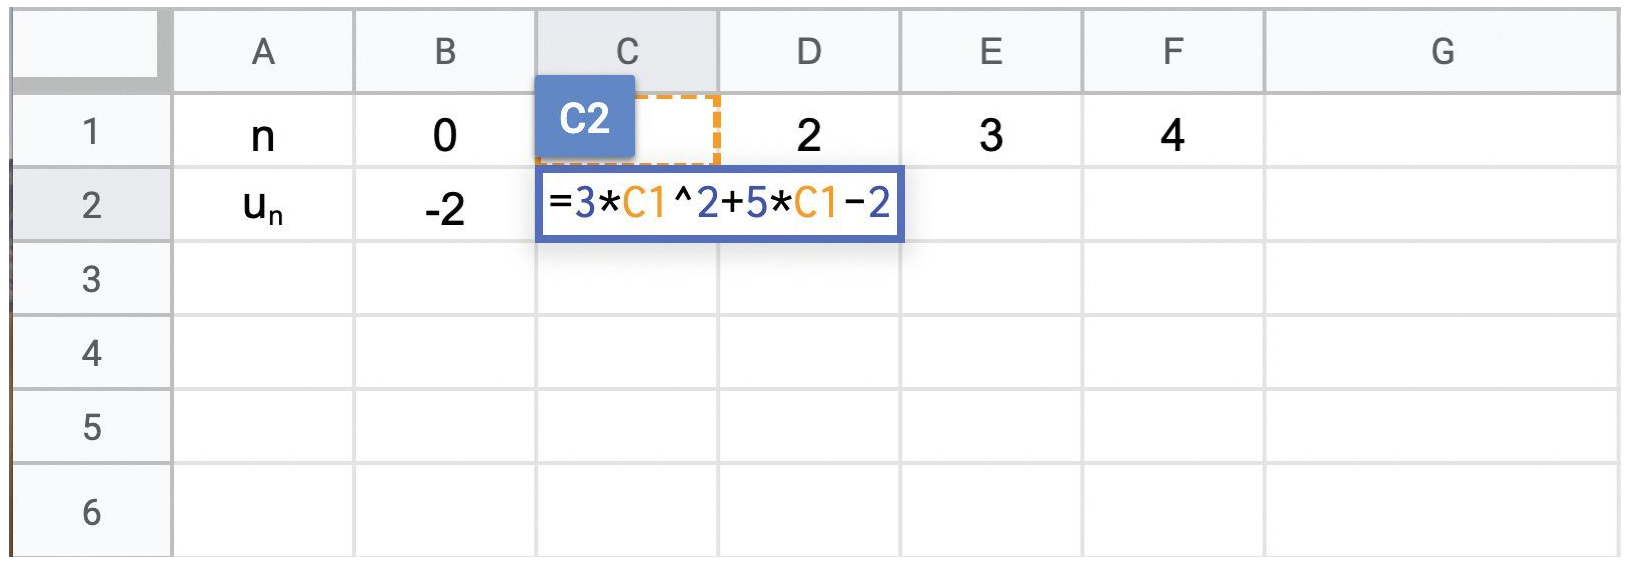
\includegraphics[width=10cm]{tableur1}
	\begin{enumalph}
		\item 	Si on étend la formule de la cellule \textbf{C2} à la cellule \textbf{D2}, quelle est la valeur de $u_2$ ?
		\item 	Exprimer le terme général $u_n$ en fonction de $n$ en utilisant la formule donnée par le tableur.
	\end{enumalph}
	\item 	Pour chacune des feuilles de calcul, écrire la relation donnant $u_{n+1}$ en fonction de $u_n$ et donner les trois premiers termes de la suite $(u_n)$.
	\begin{multicols}{2}
		\begin{enumalph}
			\item 	 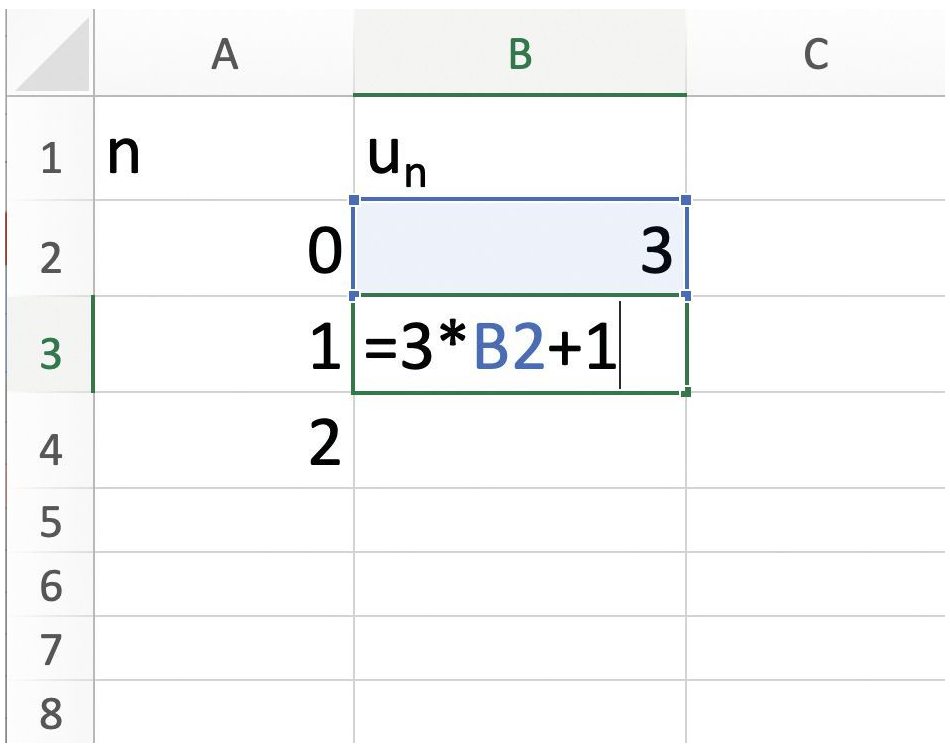
\includegraphics[width=5cm]{tableur2}
			\item 	 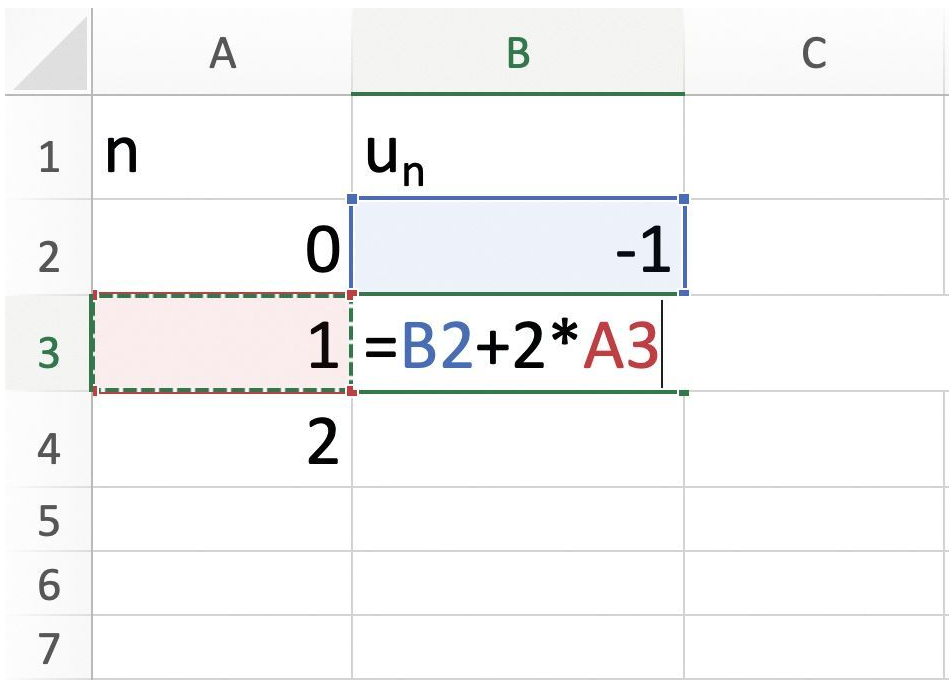
\includegraphics[width=5cm]{tableur3}
		\end{enumalph}	
	\end{multicols}
\end{enumerate}

\vspace{0.5cm}

\exo{ Suite définie par un algorithme}
\begin{multicols}{2}
	\begin{enumerate}
		\item 	On considère l'algorithme suivant:
		\begin{encadrecolore}{Algorithme}{UGLiDarkBlue}
Pour i allant de 0 à 10 : \\
\indent$\ \ \ $  u <- 2i - 1\\
Fin Pour
            \end{encadrecolore}

	\begin{enumalph}
		\item 	Quelle sera la dernière valeur calculée par cet algorithme ?
		\item 	On appelle $(u_n)$ la suite associée aux valeurs calculée par l'algorithme.\\
				Donner l'expression du terme général de cette suite.

	\end{enumalph}
    \columnbreak
		\item 	On considère le script suivant :
		\begin{pyc}
            \begin{minted}{python}
u = 1
for i in range(10) :
    u = (u-1)/(u-2)                
            \end{minted}
        \end{pyc}

		\begin{enumalph}
			
			\item 	On appelle $(u_n)$ la suite associée aux valeurs calculées par le script.\\
			\'Ecrire une relation entre $u_{n+1}$ et $u_n$ et calculer les quatre premiers termes de cette suite.
			\item À l'aide de la calculatrice, afficher les 10 premiers termes de cette suite.
		\end{enumalph}
	\end{enumerate}
\end{multicols}


\exo{ Une récurrence d'ordre 2}

La suite $r$ est définie par $r_0=2$, $r_1=3$ et, pour tout entier naturel $n$ :
$$r_{n+2}=2r_n-r_{n+1}$$
Calculer les cinq premiers termes de la suite.\\

\exo{Deux suites récurrentes imbriquées}

Les suites $a$ et $b$ sont définies par $a_0=900$, $b_0=200$ et pour tout $n\in\N$ :
$$\left\lbrace\begin{array}{llll}
	a_{n+1} & = &0,9a_n+0,1b_n \\
	b_{n+1}& = & 0,1a_n+0,9b_n\\
\end{array}
\right. $$
Calculer les trois premiers termes des deux suites.\\

\exo{Une suite périodique}

On considère la suite $p$ définie par 
$$\left\{
\begin{array}{llll}
	p_0 & = & 2 & \\
	p_{n+1} & = & 1-\dfrac{1}{p_n} & \text{pour tout } n\in\N\\
\end{array}
\right. $$

Calculer les 10 premiers termes de cette suite.


\section*{Modéliser à l'aide d'une suite}


\exo{}
On considère la succession de figures suivantes :
\begin{center}
	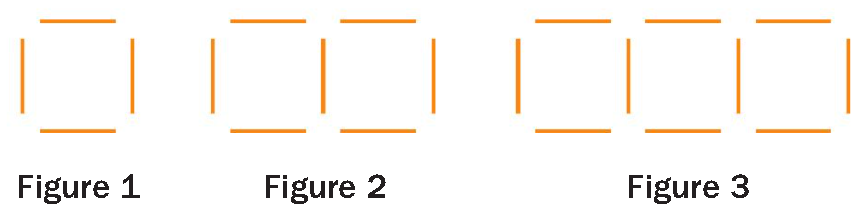
\includegraphics[width=9cm]{batons}
\end{center}
On note $b_n$ le nombre de bâtons nécessaires à la construction de la figure $n$ où $n\in\N^*$.
\begin{enumerate}
	\item 	\begin{enumalph}
		\item 	Donner les valeurs de $b_1, b_2$ et $b_3$.
		\item Tracer la figure 4 et donner la valeur de $b_4$.
		\item	Conjecturer une formule explicite de la suite $(b_n)$.	
	\end{enumalph}
	\item 	En supposant exacte la conjecture émise à la question \textbf{1c}, déterminer :
	\begin{enumalph}
		\item 	la valeur de $b_{20}$ ;
		\item 	quelle est la plus grande figure que l'on puisse construire avec 200 bâtons.
	\end{enumalph}
\end{enumerate}




\dleft{7.5cm}{
    \exo{}
    Avec des carreaux, on construit un motif géométrique par la succession des figures suivantes :
}{\begin{center}
	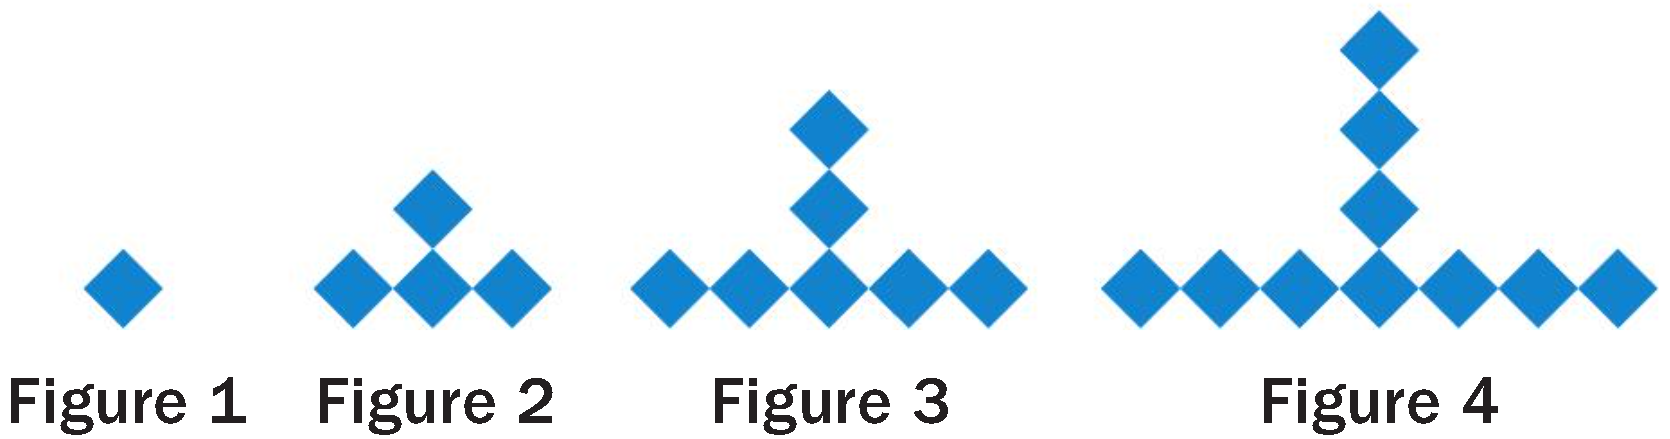
\includegraphics[width=9cm]{carreaux}
\end{center}}


Modéliser, à l'aide d'une suite récurrente, le nombre de carreaux de chaque figure.

\exo{}
En 2021, un journal régional compte 62 000 abonnés. On suppose que chaque année 85 \% des abonnés renouvellent leur abonnement et que l'on compte 4500 nouveaux abonnés.
\begin{enumerate}
	\item 	Déterminer le nombre de d'abonnés à ce journal en 2022, puis en 2023.
	\item 	Modéliser, à l'aide d'une suite récurrente, le nombre d'abonnés à ce journal.
\end{enumerate}


\exo{}
Une ville compte 195 médecins. En raison des départs à la retraite, elle enregistre chaque année une perte de médecins de 4 \% et on estime à 5 le nombre de nouveaux médecins qui s'installent.\\
À l'aide d'une suite, modéliser cette situation pour estimer le nombre de médecins dans $n$ années.\\



\dleft{8.5cm}{
\exo{}
Avec des anneaux, on réalise une succession de motifs géométriques dont on a représenté les trois premiers ci-contre.\\
Pour tout nombre entier naturel non nul $n$, on note $c_n$ le nombre d'anneaux du motif $n$.

}{\begin{center}
		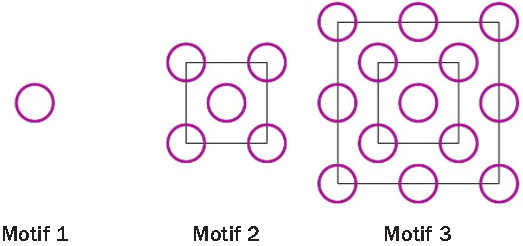
\includegraphics[width=7cm]{carres}
\end{center}}



\begin{enumerate}
	\item 	\begin{enumalph}
		\item 	Représenter le motif 4 et donner les valeurs de $c_1,c_2,c_3$ et $c_4$.
		\item 	\'Etablir une relation de récurrence entre $c_{n+1}$ et $c_n$.	
	\end{enumalph}
	\item 	On remarque que, pour tout $n\in\N^*$ : $\quad c_n=1+0\times 4+1\times 4 + ... + (n-1)\times 4$.
	\begin{enumalph}
		\item 	On admet que, pour tout $n\in\N^*$ : $\quad 1+2+...+(n-1)=\dfrac{n(n-1)}{2}$.\\
		Prouver que $\quad c_n=2n^2-2n+1$.
		\item 	Quel est le plus grand motif que l'on peut réaliser avec 2000 anneaux ?	
	\end{enumalph}
\end{enumerate}



\exo{ Suites de moyennes}
On considère les suites $(a_n)$ et $(b_n)$ vérifiant $a_0\geqslant 0, b_0\geqslant0$ et pour tout $n\in \N$ : 
$$a_{n+1}=\dfrac{a_n+b_n}{2}\quad \text{et}\quad b_{n+1}=\sqrt{a_nb_n}.$$
\begin{enumerate}
	\item 	Pour chacun des termes initiaux donnés ci-dessous:
	\begin{enumerate}[label=\textbullet]
		\item 	calculer $a_1, b_1, a_2$ et $b_2$ ;
		\item 	ranger dans l'ordre croissant les nombres $a_1, b_1, a_2$ et $b_2$.
	\end{enumerate}
	\begin{multicols}{3}
		\begin{enumalph}
			\item 	$a_0=8$ et $b_0=18$.
			\item 	$a_0=45$ et $b_0=5$.
			\item	$a_0=6$ et $b_0=6$.
		\end{enumalph}
	\end{multicols}
	
	\item 	Connaissant les nombres $a_n$ et $b_n$, une construction géométrique des nombres $a_{n+1}$ et $b_{n+1}$, sur l'axe des nombres réels d'origine O, est illustrée ci-dessous :\\
	\dleft{9.5cm}{
	\begin{enumalph}
		\item 	Justifier cette construction.\\
				\textit{Aide : Utiliser le théorème de Pythagore.}
		\item 	Conjecturer une propriété concernant la monotnie des suites $(a_n)$ et $(b_n)$.
\end{enumalph}}{\begin{center}
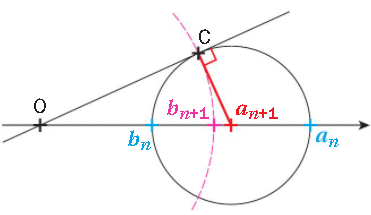
\includegraphics[width=6cm]{construction}
\end{center}}
	
\end{enumerate}
\textit{\textbf{Info :} $a$ et $b$ étant deux nombres positifs, le nombre $\sqrt{ab}$ est appelé \textbf{moyenne géométrique} de $a$ et $b$.}



\section*{Représentation graphique d'une suite}
\setlength{\columnseprule}{0.5pt}

\begin{multicols}{2}
	\exo{}
	Considérons la suite $u$ définie par :
	$$\left\{
	\begin{array}{llll}
		u_0 & = & 4 &\\ 
		u_{n+1} & = & 0,5u_n+4 & \text{pour tout } n\in\N\\
	\end{array}
	\right. $$
	\begin{enumerate}
		\item Calculer $u_1$, $u_2$, $u_3$ et $u_4$.
		\item Représenter ces termes dans le repère ci-dessous.
		\item Quelle semblent être la variation et la « limite » de la suite $u$ ?
	\end{enumerate}
	\begin{tikzpicture}
		\reperev{-1}{-1}{5}{9}
	\end{tikzpicture}

	\exo{}
	Considérons la suite $v$ définie par :
	$$\left\{
	\begin{array}{llll}
		v_0 & = & 16 &\\ 
		v_{n+1} & = & 0,5v_n+4 & \text{pour tout } n\in\N\\
	\end{array}
	\right. $$
	\begin{enumerate}
		\item Calculer $v_1$, $v_2$, $v_3$ et $v_4$.
		\item Représenter ces termes dans le repère ci-dessous.
		\item Quelle semblent être la variation et la « limite » de la suite $v$ ?
	\end{enumerate}
	
	\begin{tikzpicture}[yscale=.5]
		\reperev{-1}{-1.5}{5}{18}
	\end{tikzpicture}
\end{multicols}

\setlength{\columnseprule}{0pt}


\exo{}
On considère la famille de suites $(\alpha_n)$ suivante :
$\left\{
\begin{array}{llll}
	\alpha_0 & = & a & \text{où } a \text{ est un réel donné}\\ 
	\alpha_{n+1} & = & 0,5\alpha_n+4 & \text{pour tout } n\in\N\\
\end{array}
\right. $\\[.5em]
Il existe un moyen commode de représenter ces suites :
\begin{enumerate}[label=\textbullet]
	\item 	On pose pour tout $x\in\R$, $f(x)=0,5x+4$.
	\item 	Dans un repère \textbf{orthogonal}, on représente $\mathcal{C}_f$ et la droite d'équation $y=x$ :	
\end{enumerate}


\def\xmin{-1} \def\ymin{-1}\def\xmax{16}\def\ymax{12}
\def\F{0.5*\x+4)}
\begin{tikzpicture}
	\clip (\xmin,\ymin) rectangle (\xmax,\ymax);
	\draw[fill = white] (\xmin,\ymin) rectangle (\xmax,\ymax);
	\repereal{\xmin}{\ymin}{\xmax}{\ymax}
	\draw[thick,color=gray,domain=\xmin:\xmax,smooth,variable=\x] plot ({\x},{\x});	
	\draw[thick,domain=\xmin:\xmax,smooth,variable=\x] plot ({\x},{\F});	
	
\end{tikzpicture}

\begin{enumerate}
	\item 	On considère la suite $u$ définie à l'exercice 14.\\
	Au crayon à papier (puis en rouge une fois que vous êtes sûr(e) de vous) nous allons représenter les premiers termes de $u$ :
	\begin{enumerate}[label=\textbullet]
		\item 	Placer sur l'axe des abscisses le \textbf{nombre} $u_0$.
		\item 	Placer le \textbf{point} de coordonnées $\pc{}{u_0}{f(u_0)}$.
		\item 	Placer le \textbf{point} de coordonnées $\pc{}{f(u_0)}{f(u_0)}$ et relier avec le \textbf{point} précédent.
		\item 	Puisque $f(u_0)=u_1$, placer sur l'axe des abscisses le \textbf{nombre} $u_1$.
		\item 	Placer le \textbf{point} de coordonnées $\pc{}{u_1}{f(u_1)}$ et relier avec le \textbf{point} précédent.
		\item 	Placer le \textbf{point} de coordonnées $\pc{}{f(u_1)}{f(u_1)}$ et relier avec le \textbf{point} précédent.
		\item 	Puisque $f(u_1)=u_2$, placer sur l'axe des abscisses le \textbf{nombre} $u_2$.
		\item 	Et c\ae tera.
	\end{enumerate}
	\item 	Faire de même en vert pour les premiers termes de la suite $v$ définie à l'exercice 15.
\end{enumerate}



\exo{}
On peut adapter ce procédé aux suites définies par récurrence à l'aide d'une fonction $f$ :
$$\left\{
\begin{array}{llll}
	u_0 & = & a & \text{où } $a$\text{ est un réel donné}\\ 
	u_{n+1} & = & f(u_n) & \text{pour tout } n\in\N\\
\end{array}
\right. $$

Pour l'exemple, prenons $f$ définie sur $\fii{-1}$ par $f(x)=\sqrt{1+x}$.\\
Représenter sans chercher à les calculer, les premiers termes de la suite $r$ définie par

$$\left\{
\begin{array}{llll}
	r_0 & = & 8 & \\ 
	u_{n+1} & = & \sqrt{1+r_n} & \text{pour tout } n\in\N\\
\end{array}
\right. $$

%\vspace{0.5cm}

\def\xmin{-.5} \def\ymin{-.5}\def\xmax{8}\def\ymax{4}
\def\F{(\x+1)^(.5)}
\begin{tikzpicture}[scale=2]
	\clip (\xmin,\ymin) rectangle (\xmax,\ymax);
	\draw[fill = white] (\xmin,\ymin) rectangle (\xmax,\ymax);
	\repereal{\xmin}{\ymin}{\xmax}{\ymax}
	\draw[thick,color=gray,domain=\xmin:\xmax,smooth,variable=\x] plot ({\x},{\x});	
	\draw[thick,domain=\xmin:\xmax,smooth,variable=\x] plot ({\x},{\F});		
\end{tikzpicture}	

\begin{enumerate}
	\item 	Conjecturer la variation de $r$ et donner une valeur approchée de sa limite.
	\item 	Proposer une valeur exacte en déterminant l'intersection de $\mathcal{C}_f$ et de la droite d'équation $y=x$.
\end{enumerate}


\newpage

\exo{}

Faire de même avec 
$\quad \left\{
\begin{array}{llll}
	q_0 & = & 7 & \\ 
	q_{n+1} & = &\dfrac{4}{1+q_n} & \text{pour tout } n\in\N\\
\end{array}
\right. $
\begin{center}
	\def\xmin{-1} \def\ymin{-1}\def\xmax{8}\def\ymax{4}
	\def\F{4/(1+\x)}
	\begin{tikzpicture}[scale=2]
		\clip (\xmin,\ymin) rectangle (\xmax,\ymax);
		\draw[fill = white] (\xmin,\ymin) rectangle (\xmax,\ymax);
		\repereal{\xmin}{\ymin}{\xmax}{\ymax}
		\draw[thick,color=gray,domain=\xmin:\xmax,smooth,variable=\x] plot ({\x},{\x});	
		\draw[thick,domain=-.9:\xmax,smooth,variable=\x] plot ({\x},{\F});	
	\end{tikzpicture}\ \\
\end{center}





\exo{}

De même avec 
$\quad \left\{
\begin{array}{llll}
	v_0 & = & 2 &  \\ 
	v_{n+1} & = &1-\dfrac{1}{v_n} & \text{pour tout } n\in\N\\
\end{array}
\right. $
\begin{center}
	\def\xmin{-2} \def\ymin{-2}\def\xmax{4}\def\ymax{4}
	\def\F{1-1/\x}
	\begin{tikzpicture}[scale=1.5]
		\clip (\xmin,\ymin) rectangle (\xmax,\ymax);
		\draw[fill = white] (\xmin,\ymin) rectangle (\xmax,\ymax);
		\repereal{\xmin}{\ymin}{\xmax}{\ymax}
		\draw[thick,color=gray,domain=\xmin:\xmax,smooth,variable=\x] plot ({\x},{\x});	
		\draw[thick,domain=\xmin:-.1,smooth,variable=\x] plot ({\x},{\F});
		\draw[thick,domain=.1:\xmax,smooth,variable=\x] plot ({\x},{\F});		
	\end{tikzpicture}
\end{center}	


\section*{Sens de variation}

Dans chaque cas, étudier le sens de variation de la suite $(u_n)$ définie par la relation donnée.

\exo{ À l'aide d'une étude de fonction}
\begin{multicols}{2}
	\begin{enumerate}
		\item 	Pour tout $n\in\N$, $u_n=3n-4$
		\item 	Pour tout $n\in\N$, $u_n=3n^2-4$
		\item 	Pour tout $n\in\N$, $u_n=-2n-3$
		\item 	Pour tout $n\in\N$, $u_n=n^2-10n+15$
	\end{enumerate}
\end{multicols}


\exo{ À l'aide du signe de $u_{n+1}-u_n$}
\begin{multicols}{2}
	\begin{enumerate}
		\item 	Pour tout $n\in\N$, $u_n=2n^2-n+1$
		\item 	$\left\{
		\begin{array}{llll}
			u_0 & = & 2 &\\ 
			u_{n+1} & = & u_n-\sqrt{u_n^2+3} & \text{pour tout}\ n\in\N\\
		\end{array}\right. $\\
	
		\columnbreak
		\item 	$\left\{
		\begin{array}{llll}
			u_0 & = & 1 &\\ 
			u_{n+1} & = & -u_n^2+u_n-1 &\text{pour tout}\ n\in\N\\
		\end{array}\right. $
		\item 	$\left\{
		\begin{array}{llll}
			u_0 & = & 3 &\\ 
			u_{n+1} & = & u_n+n^2-n+3&\text{pour tout}\  n\in\N\\
		\end{array}\right. $
	\end{enumerate}
\end{multicols}

\exo{ Sens de variation d'une suite à termes positifs à l'aide de $\dfrac{u_{n+1}}{u_n}$}
On admet que les suites $u,v$ et $w$ sont à termes strictement positifs.
\begin{enumalph}
	\item 	$u$ définie par $u_0=20$ et pour tout $n\in\N$, $u_{n+1}=1,4u_n$.
	\item 	$v$ définie par $v_0=1$ et pour tout $n\in\N$, $v_{n+1}=\dfrac{v_n}{n+1}$.
	\item 	$w$ définie pour tout $n\in\N^*$ par , $w_{n}=\dfrac{n}{2^n}$.
\end{enumalph}

\exo{}
\begin{multicols}{2}
	\begin{enumerate}
		\item 	Pour tout $n\in\N$, $u_n=2n^2-n+1$
		\item 	Pour tout $n\in\N$, $v_n=(4n-1)^2$
		\item 	Pour tout $n\in\N^*$, $w_n=1+\dfrac{1}{2}+\dfrac{1}{3}+\ldots+\dfrac{1}{n}$
		\item 	Pour tout $n\in\N$, $x_n=1+2^2+3^3+\ldots+n^n$
	\end{enumerate}
	
\end{multicols}


\exo{}
\begin{multicols}{2}
	\begin{enumerate}
		\item 	Pour tout $n\in\N$, $u_n=(-1)^n$
		\item 	Pour tout $n\in\N$, $v_n=5n^2-n+2$\\
		\columnbreak
		
		\item 	$\left\{
		\begin{array}{llll}
			t_0 & = & 2 &\\ 
			t_{n+1} & = & t_n-(n+3)^2&\text{pour tout}\  n\in\N\\
		\end{array}\right. $
		\item 	$\bigstar$ Pour tout $n\in\N$, $w_n=n^3+7n+3$
	\end{enumerate}
\end{multicols}
Pour la question \textbf{4.}, on pourra utiliser l'identité :$\quad (a+b)^3=a^3+3a^2b+3ab^2+b^3$.\\


\newpage

\exo{}
\begin{multicols}{2}
	\begin{enumerate}
		\item 	Pour tout $n\in\N$, $u_n=9n+(-3)^n$
		\item 	Pour tout $n\in\N$, $v_n=n^3-n^2$\\
		\item 	Pour tout $n\in\N$, $w_n=1+\dfrac{1}{n+1}$
		\item 	$\left\{
		\begin{array}{llll}
			t_0 & = & 2 &\\ 
			t_{n+1} & = & t_n-\sqrt{n+1}& \text{pour tout }  n\in\N\\
		\end{array}\right. $
	\end{enumerate}
\end{multicols}




\end{document}